%==============================================================================
% Document header
%==============================================================================
\documentclass[a4paper,11pt]{article}

% Color package
\usepackage[usenames,dvipsnames,table]{xcolor}

% Hyperrefs
\usepackage[
  colorlinks = true,
  linkcolor  = Mahogany,
  citecolor  = Mahogany,
  urlcolor   = blue,
]{hyperref}

\usepackage{graphicx}
\usepackage{rotating}
\usepackage{multirow}

\usepackage{longtable}

% Header and footer customization
\usepackage{fancyhdr}
\pagestyle{fancy}
\fancyhead[L]{\nouppercase{\leftmark}}
\fancyhead[R]{} 
\renewcommand{\footrulewidth}{0.4pt}

%==============================================================================
% Start of document
%==============================================================================
\begin{document}

%------------------------------------------------------------------------------
% Title
%------------------------------------------------------------------------------
\begin{titlepage}

\vspace*{3cm}

\noindent{\LARGE \textbf{I$^2$C Slave Core}}

\noindent \rule{\textwidth}{.1cm}

\hfill\today

\vspace*{3cm}

\begin{figure}[h]
  
\includegraphics[height=3cm]{fig/cern-logo}
  \hfill
  
\includegraphics[height=3cm]{fig/ohwr-logo}
\end{figure}

\vfill

\noindent {\Large \textbf{Theodor-Adrian Stana (CERN/BE-CO-HT)}}

\noindent \rule{\textwidth}{.05cm}

\end{titlepage}


%------------------------------------------------------------------------------
% Revision history
%------------------------------------------------------------------------------
\thispagestyle{empty}
\section*{Revision history}

\centerline
{
  \rowcolors{2}{white}{gray!25}
  \begin{tabular}{l c p{.6\textwidth}}
  \hline
  \multicolumn{1}{c}{\textbf{Date}} & \multicolumn{1}{c}{\textbf{Version}} & \multicolumn{1}{c}{\textbf{Change}} \\
  \hline
  03-03-2014 & 0.01 & First draft \\
  \hline
  \end{tabular}
}

%------------------------------------------------------------------------------
% Generate TOC and pagebreak after it
%------------------------------------------------------------------------------
\pagebreak
\pagenumbering{roman}
\setcounter{page}{1}
\tableofcontents

%------------------------------------------------------------------------------
% List of figs, tables, abbrevs
%------------------------------------------------------------------------------
\listoffigures
\listoftables

%------------------------------------------------------------------------------
% List of abbreviations
%------------------------------------------------------------------------------
\pagebreak
\section*{List of Abbreviations}
\begin{tabular}{l l}
FF & Flip-Flop \\
\end{tabular}

%==============================================================================
% SEC: Intro
%==============================================================================
\pagebreak
\pagenumbering{arabic}
\setcounter{page}{1}
\section{Introduction}
\label{sec:intro}

This document presents the \textit{gc\_glitch\_filt} component, a modular glitch
filter open-hardware~\cite{ohwr} design for FPGA or ASIC implementation. It is
implemented as one short VHDL file which can be found under the following folder
of the \textit{general-cores} repository~\cite{gencores-ohwr}:

\begin{itemize}
\item \textit{modules/common/}
\end{itemize}

%==============================================================================
% SEC: Instantiation
%==============================================================================
\section{Instantiation}
\label{sec:instantiation}

Table~\ref{tbl:ports} shows the instantiation template for the \textit{gc\_glitch\_filt}
component. It can be directly instantiated in a VHDL or Verilog design.

The data to be filtered should be connected to the \textit{dat\_i} input. Note that
the data is not synchronized internally to the \textit{clk\_i} signal, if metastability
is a concern, a synchronization chain should be provided outside the component.

The deglitched data is presented at the \textit{dat\_o} output a number of \textit{g\_len+1}
clock cycles later.

\begin{table}[h]
  \caption{Ports and generics of \textit{gc\_i2c\_slave} module}
  \label{tbl:ports}
  \centerline
  {
    \rowcolors{2}{white}{gray!25}
    \begin{tabular}{l p{.7\textwidth}}
      \hline
      \multicolumn{1}{c}{\textbf{Name}} & \multicolumn{1}{c}{\textbf{Description}} \\
      \hline
      g\_len & Glitch filter length generic (in \textit{clk\_i} cycles) \newline
               1 -- glitches narrower than 1 \textit{clk\_i} cycle are filtered \newline
               2 -- glitches narrower than 2 \textit{clk\_i} cycles are filtered \newline
               etc.\\
      \hline
      clk\_i & Clock input \\
      rst\_n\_i & Active-low reset input \\
      dat\_i & Data input (should be synchronous to \textit{clk\_i})\\
      dat\_o & Deglitched data output (synchronous to \textit{clk\_i}) \\
      \hline
    \end{tabular}
  }
\end{table}

%==============================================================================
% SEC: implem
%==============================================================================
\pagebreak
\section{Implementation and operation}

Figure~\ref{fig:implem} shows the implementation of the \textit{gc\_glitch\_filt}
block.

\begin{figure}[h]
  \centerline{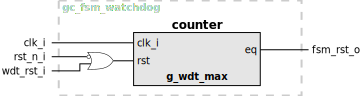
\includegraphics[width=\textwidth]{fig/implem}}
  \caption{Implementation of the \textit{gc\_glitch\_filt} block}
  \label{fig:implem}
\end{figure}

The block's operation is very simple and can be summarized as follows. At synthesis
time, \textit{g\_len} FFs are generated. If the \textit{dat\_i} is stable for a number
of \textit{g\_len} cycles, all FFs in the deglitching stage have the same value,
and the \textit{dat\_o} output changes to reflect the state of \textit{dat\_i}.
Should a glitch occur at any time on the \textit{dat\_i} signal, it is filtered
by the AND (or NAND) gate at the output.

All the FFs are cleared ('0') on reset.

%==============================================================================
% Bibliography
%==============================================================================
\pagebreak
\bibliographystyle{ieeetr}
\bibliography{gc_glitch_filt}

\end{document}
